\documentclass[12pt]{article}
\usepackage{geometry}
\geometry{margin=0.9in}
\usepackage{tikz}
\usepackage{enumitem}
\usepackage{parskip}
\usepackage{xcolor}
\definecolor{isaorange}{HTML}{C2410C}

\newcommand{\bigtask}[1]{\par\medskip\noindent{\large\textbf{\color{isaorange}#1}}\par}

% A box with a dashed line down the middle, for "draw half, then complete it".
\newcommand{\mirrorbox}[1]{%
  \par\vspace{4pt}\noindent
  \begin{tikzpicture}
    \draw[rounded corners, line width=1pt] (0,0) rectangle (\linewidth,#1);
    \draw[dashed, gray, line width=1pt] (0.5\linewidth,0) -- (0.5\linewidth,#1);
    \node[gray] at (0.5\linewidth, -0.35) {\footnotesize fold line};
  \end{tikzpicture}\par\vspace{10pt}}

% Pattern-row shapes (all the same size, sitting on the same baseline).
\newcommand{\pcirc}[1]{\draw[fill=blue!25, line width=0.8pt] (#1,0) circle (0.42);}
\newcommand{\psq}[1]{\draw[fill=orange!35, line width=0.8pt] (#1-0.42,-0.42) rectangle (#1+0.42,0.42);}
\newcommand{\pblank}[1]{\draw[dashed, line width=0.9pt] (#1-0.42,-0.42) rectangle (#1+0.42,0.42);}

% A triangle of dots: #1 rows (1 on top, #1 on the bottom), color #2.
\newcommand{\tritile}[2]{%
  \foreach \r in {1,...,#1}{%
    \foreach \c in {1,...,\r}{%
      \pgfmathsetmacro{\xx}{((\c-1) - (\r-1)/2)*0.55}%
      \pgfmathsetmacro{\yy}{(#1-\r)*0.55}%
      \fill[#2] (\xx,\yy) circle (0.13);%
    }%
  }%
}

\begin{document}

\begin{center}
  {\huge\textbf{Patterns and What Comes Next}}\\[2pt]
  {\large Find the rule, then guess what comes next}
\end{center}
\vspace{0.3cm}

\bigtask{1. Keep the pattern going}
Draw the next 3 shapes in each row so the pattern keeps going.
\begin{center}
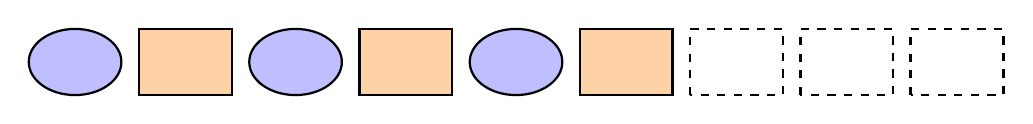
\begin{tikzpicture}[x=1.4cm]
  \pcirc{0}\psq{1}\pcirc{2}\psq{3}\pcirc{4}\psq{5}
  \pblank{6}\pblank{7}\pblank{8}
\end{tikzpicture}
\end{center}

\begin{center}
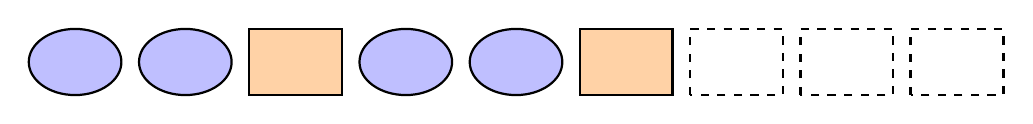
\begin{tikzpicture}[x=1.4cm]
  \pcirc{0}\pcirc{1}\psq{2}\pcirc{3}\pcirc{4}\psq{5}
  \pblank{6}\pblank{7}\pblank{8}
\end{tikzpicture}
\end{center}

\bigtask{2. The growing triangles}
Step 1 has 1 dot. Step 2 has 3 dots. Step 3 has 6 dots. Draw step 4 in the empty box.
\begin{center}
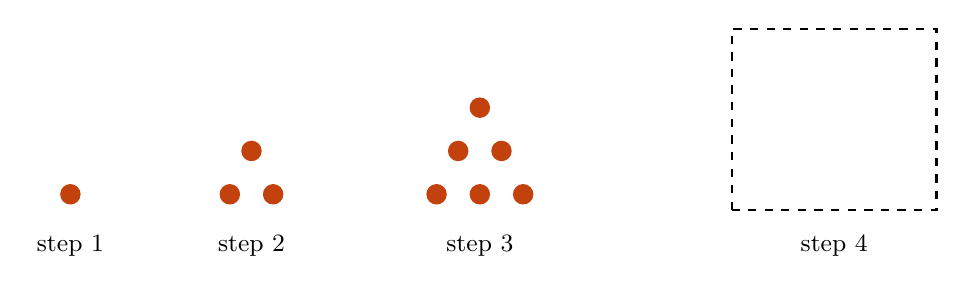
\begin{tikzpicture}
  \begin{scope}[xshift=0cm]\tritile{1}{isaorange}\end{scope}
  \begin{scope}[xshift=2.3cm]\tritile{2}{isaorange}\end{scope}
  \begin{scope}[xshift=5.2cm]\tritile{3}{isaorange}\end{scope}
  \draw[dashed, line width=0.9pt] (8.4,-0.2) rectangle (11.0,2.1);
  \node at (0,-0.65) {\small step 1};
  \node at (2.3,-0.65) {\small step 2};
  \node at (5.2,-0.65) {\small step 3};
  \node at (9.7,-0.65) {\small step 4};
\end{tikzpicture}
\end{center}
Step 4 has \underline{\hspace{2cm}} dots. \qquad Step 5 has \underline{\hspace{2cm}} dots.

\bigtask{3. Doubling}
Each number is twice the one before. Fill in the last two.
\begin{center}
  {\Large 1 \quad 2 \quad 4 \quad 8 \quad \underline{\hspace{1.6cm}} \quad \underline{\hspace{1.6cm}}}
\end{center}

\bigtask{4. Make your own pattern}
Draw a pattern of your own in the boxes. Then tell a grown-up your rule.
\begin{center}
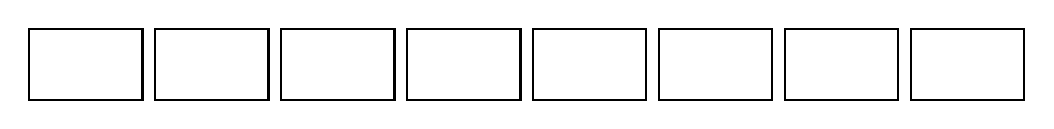
\begin{tikzpicture}[x=1.6cm]
  \foreach \i in {0,1,2,3,4,5,6,7}{
    \draw[line width=0.9pt] (\i-0.45,-0.45) rectangle (\i+0.45,0.45);
  }
\end{tikzpicture}
\end{center}
My rule is: \hrulefill

\end{document}
